\paragraph{Menus}

    Pour lancer une partie, il faut sélectionner \textit{Play} dans le menu principal. Si c'est la première fois que vous lancez le jeu, 
    une fenêtre vous proposera de lancer le tutoriel pour apprendre à jouer. Si vous sélectionnez Jouer en ligne, vous passez le tutoriel. 
    Vous aurez ensuite accès à un champ \textit{Pseudo}, qui vous permet de choisir votre pseudonyme en jeu. Vous avez ensuite trois possibilités :

    \begin{figure}[hbt!]
        \centering
        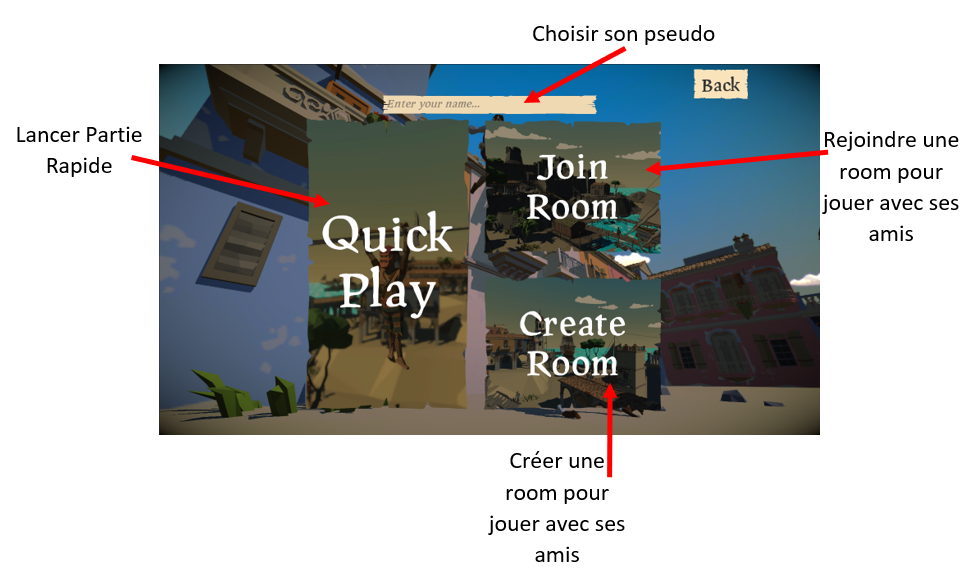
\includegraphics[scale=0.435]{main.png}
        \caption{Menu de choix du mode de jeu}
    \end{figure}
    \FloatBarrier

    \paragraph{}
    Partie rapide (Quick Play), qui vous permet de rejoindre directement une partie ouverte. Vous jouerez donc avec des 
    inconnus sur un lobby aléatoire.

    \paragraph{}
    Créer une partie : Cette option vous permet, comme son nom l'indique, de créer une partie. Par défaut, cette dernière 
    sera publique (ouverte à tous les joueurs), mais vous pouvez sélectionner la coche \textit{partie privée} pour rendre 
    le salon accessible uniquement à l'aide d'un code qui apparaît alors sur votre écran.

    \begin{figure}[hbt!]
        \centering
        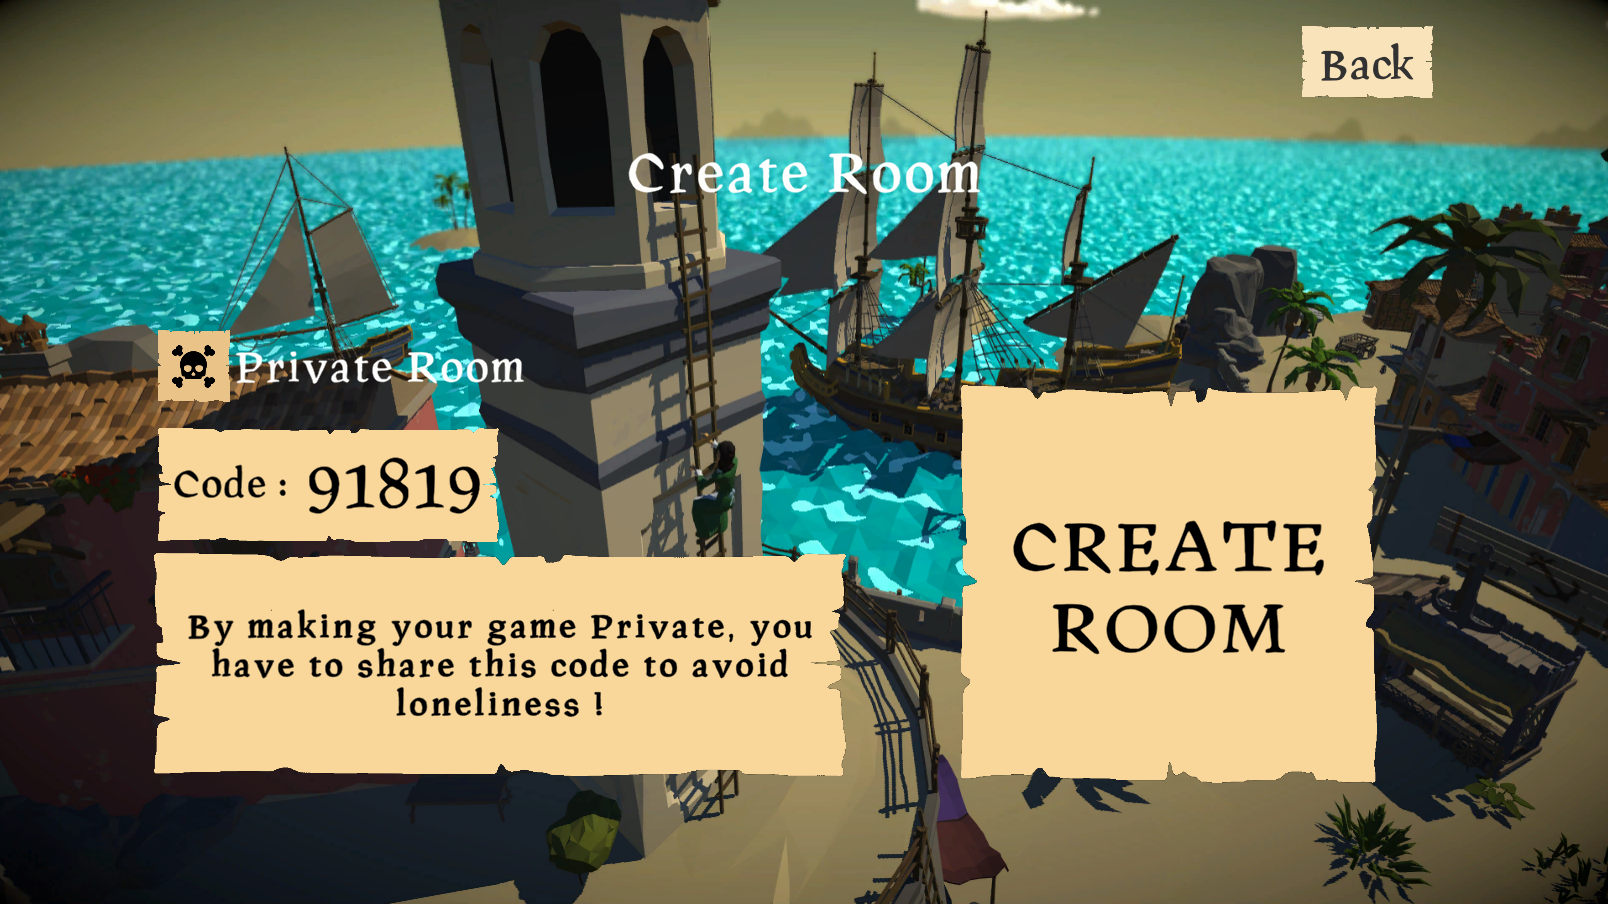
\includegraphics[scale=0.18]{private.png}
        \caption{Menu de création de parties}
    \end{figure}
    \FloatBarrier

    \paragraph{}
    Rejoindre une partie : Ce menu permet de rejoindre des parties privées en renseignant leur code.

    \begin{figure}[hbt!]
        \centering
        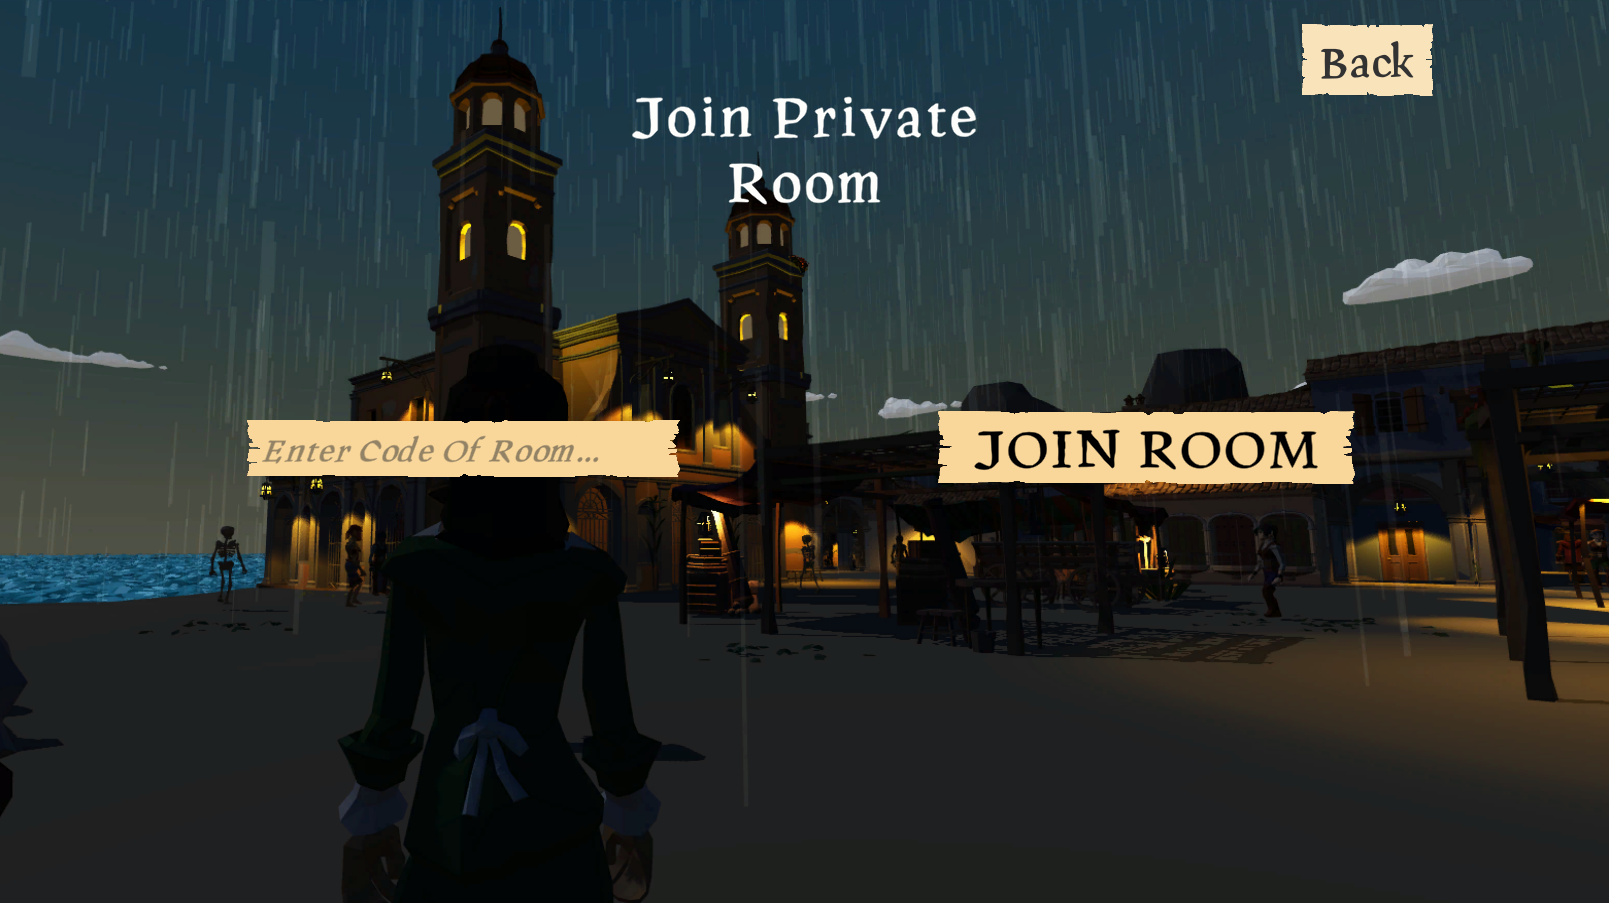
\includegraphics[scale=0.18]{public.png}
        \caption{Menu pour rejoindre une partie}
    \end{figure}
    \FloatBarrier


\paragraph{Lobby}

    Sur le lobby (salle d'attente de la partie), le joueur est invité à choisir sa classe de personnage, et à 
    patienter en faisant le parcours de saut ou en discutant via le chat intégré. Les parties se lancent lorsque quatre joueurs au moins 
    se connectent. Un décompteur de dix secondes est alors lancé, à l'issue duquel la partie est lancée.

    